\section{Fourier Transform}
%==============================================%
\subsection{From Fourier Series to Fourier Transform}
\begin{ex}{}
    To find a representation of any finite energy signal, not necessarily periodic: \underline{set the periodical of a period signal to \textit{infinity}}.\\
    
    \boxed{\begin{minipage}{0.3\textwidth}
        \[ 
        x(t) = 
        \begin{cases}
        1,  & \lvert t \rvert<T_{1} \\
        0,  & T_{1}<\lvert t \rvert<\frac{T}{2}\\
        \end{cases} 
        \] 
    \end{minipage} \hfill
    \begin{minipage}{0.7\textwidth}
        \begin{figure}[H] 
            \centering
            \includegraphics[width = 0.9\textwidth]{images/T1} 
        \end{figure} 
    \end{minipage}}\\\\
    
    \begin{wrapfigure}{R}{0.5\textwidth}
        \includegraphics[width = 0.45\textwidth]{images/tincrease} \vspace{-3cm} 
    \end{wrapfigure}
    
    The Fourier series of the periodic signal $x(t)$ above is:
    \[ 
    x(t) =  \sum_{k=-\infty}^{\infty} \ c_{k} e^{j\frac{2\pi k}{T}t}
    \]
    with
    \begin{align*}
    \begin{split}
        c_{k} 
        &= \frac{1}{T} \int_{-T_{1}}^{T_{1}} x(t)e^{-j\frac{2\pi k}{T}t} \\
        &= \frac{2 \sin(k \omega_{0} T_{1})}{k \omega_{0} T} \\
        &=\frac{1}{T} \ \frac{2 \sin(\omega T_{1})}{\omega} \bigg\rvert_{\omega = k \omega_{0}} 
    \end{split} 
    \end{align*}\\
    where $\omega_{0}=\frac{2\pi}{T}$ is the frequency of the first harmonic.\\\\
    Plot $c_{k}$ against $\omega$. As $T$ increases, the frequency becomes smaller, and the points on the plot become closer.\\
    
    Generalize the example above:\\
    The signal $x(t)$ defined in the interval $t \in [-T_{1}, T_{1}]$. We build the corresponding periodic signal $\tilde{x}(t)$, which equals to $x(t)$ in one period. As $T \to \infty$, $\tilde{x}(t) \to x(t)$.
    \begin{figure}[H] 
        \centering 
        \includegraphics[width = 0.6\textwidth]{images/tildex} 
    \end{figure}
    
    \[ 
        \tilde{x}(t) = \sum_{k=-\infty}^{\infty} \ c_{k} \ e^{j\frac{2\pi k}{T}t} 
    \]
    \quad with
    \begin{align*}
    \begin{split}
        c_{k} 
        &= \frac{1}{T} \int_{\frac{T}{2}}^{-\frac{T}{2}} \tilde{x}(t)e^{-j\frac{2\pi k}{T}t} dt \\
        &= \frac{1}{T} \underbrace{\int_{-\infty}^{+\infty} x(t)e^{-j k \omega_{0} t} dt}_{X(k\omega_{0})}\\
        &=\frac{1}{T} X(k\omega_{0}) 
    \end{split}
    \end{align*}
    \textbf{ $x(t) \to X(\omega)$ is known as Fourier transform.}
    
    \begin{align*}
    \begin{split}
        \tilde{x}(t) &=\sum_{k=-\infty}^{\infty} \ c_{k} \ e^{j\frac{2\pi k}{T}t}\\
        &= \sum_{k=-\infty}^{\infty}  \ \frac{1}{T} X(k\omega_{0}) e^{j\frac{2\pi k}{T}t}\\
        &= \frac{1}{2 \pi} \ \sum_{k=-\infty}^{\infty} \ X(k \omega_{0}) \ e^{j k \omega_{0} t} \ \omega_{0} 
    \end{split}
    \end{align*}
    As $T \to \infty$, $\tilde{x}(t) \to x(t)$, $\omega_{0} \to 0$:
    \begin{equation}
        \tilde{x}(t) = x(t) = \frac{1}{2 \pi} \ \int_{-\infty}^{\infty} \ X( \omega) \ e^{j \omega t} \ d\omega 
    \end{equation}
    \textbf{$X(\omega) \to x(t)$ is known as inverse Fourier transform.}
\end{ex}

%==============================================%
\subsection{The Continuous-time Fourier Transform}
\textbf{Fourier transform:}
\[ X(\omega) =  \int_{-\infty}^{+\infty} x(t) \ e^{-j \omega t} dt \]
\textbf{Inverse Fourier transform:}
\[ x(t) = \frac{1}{2 \pi} \ \int_{-\infty}^{\infty} \ X( \omega) \ e^{j \omega t} \ d\omega \]

\begin{itemize}
    \item Fourier transform is a mathematical transformation employed to transform signals between the time domain and the frequency domain.
    
    \item Fourier transform is a reversible operation.
    
    \item \textbf{Fourier transform is a linear transformation}: it is defined by an integral
    
    \item For each value of $\omega$, the Fourier transform is a complex number representing the projection of the signal on the complex exponential function $e^{j \omega t }$.
    \[ X(\omega) = \langle x(t), e^{j \omega t} \rangle \]
    
    \item \textbf{The Fourier transform exists for signals in the $L^{2}$ space.} These signals can be expressed as the combination of functions $e^{j \omega t}$.
\end{itemize}

\begin{tcolorbox}[title=Compare Fourier series and Fourier transform, breakable]
    Fourier series:
    \[ 
    x(t) =  \sum_{k=-\infty}^{\infty} \ c_{k} \ e^{j\frac{2\pi k}{T}t} \quad with \quad c_{k} = \frac{1}{T} \int_{0}^{T} x(t) \ e^{-j\frac{2\pi k}{T}t} 
    \]
    Fourier transform:
    \[ 
    x(t) = \frac{1}{2 \pi} \ \int_{-\infty}^{+\infty} \ X( \omega) \ e^{j \omega t} \ d\omega 
    \]
    \[ 
    X(\omega) =  \int_{-\infty}^{+\infty} x(t) \ e^{-j \omega t} \ dt 
    \]
    The Fourier series represent \textit{periodic} signals with \textit{discrete} frequencies; the Fourier transform represents \textit{non-periodic} signals with \textit{continuous} frequencies.
\end{tcolorbox}

%==============================================%
\subsection{Properties of Fourier Transform}

\subsubsection{Linearity}
\[ \mathcal{FT} \{ a_{1}x_{1}(t)+a_{2}x_{2}(t)\} = a_{1}X_{1}(\omega)+a_{2}X_{2}(\omega) \]
\begin{dv}{}
    Given
    \[ 
    X_{1}(\omega) =  \int_{-\infty}^{+\infty} x_{1}(t) \ e^{-j \omega t} \ dt \quad \text{and} \quad X_{2}(\omega) =  \int_{-\infty}^{+\infty} x_{2}(t) \ e^{-j \omega t} \ dt 
    \]
    \begin{align*}
    \begin{split}
        \mathcal{FT} \{ a_{1}x_{1}(t)+a_{2}x_{2}(t) \} 
        &= \int_{-\infty}^{+\infty} \big( a_{1}x_{1}(t)+a_{2}x_{2}(t)\big) \ e^{-j \omega t} \ dt  \\
        &= a_{1}\int_{-\infty}^{+\infty}x_{1}(t)e^{-j \omega t} \ dt + a_{2}\int_{-\infty}^{+\infty}x_{2}(t) e^{-j \omega t} \ dt \\
        &= a_{1}X_{1}(\omega)+a_{2}X_{2}(\omega)
    \end{split} 
    \end{align*} 
\end{dv}

\subsubsection{Time shifting}
\[ \mathcal{FT} \{ x(t-t_{0}) \} = e^{-j \omega t_{0}}\mathcal{FT} \{ x(t)\} = e^{-j \omega t_{0}} \ X(\omega) \]
\begin{dv}{}
    \[ \mathcal{FT} \{ x(t-t_{0}) \} =  \int_{-\infty}^{+\infty} x(t-t_{0}) \ e^{-j \omega t} \ dt\] 
    Let $r = t - t_{0}$:
    \begin{align*}
    \begin{split}
        \mathcal{FT} \{ x(t-t_{0}) \} &=  \int_{-\infty}^{+\infty} x(r) \ e^{-j \omega (r+t_{0})} \ dr\\
        &= \int_{-\infty}^{+\infty} x(r) \ e^{-j \omega r} \ e^{-j \omega t_{0}} dr \\
        &= e^{-j \omega t_{0}} \ \int_{-\infty}^{+\infty} x(r) \ e^{-j \omega r}dr 
    \end{split} 
    \end{align*}
    Let $r = t$:
    \begin{align*}
    \begin{split}
        \mathcal{FT} \{ x(t-t_{0}) \} &= e^{-j \omega t_{0}} \ \underbrace{\int_{-\infty}^{+\infty} x(t) \ e^{-j \omega t} dt}_{\text{Fourier Transform}}\\
        & = e^{-j \omega t_{0}}\mathcal{FT} \{ x(t)\}\\
        &=e^{-j \omega t_{0}} \ X(\omega)
    \end{split} 
    \end{align*}
\end{dv}

\subsubsection{Conjugation}
\[ \mathcal{FT} \{ x^{*}(t)\} = X^{*}(-\omega) \]
\ if $x(t)$ is real, $X(-\omega) = X^{*}(\omega)$.
\begin{dv}{}
    The Fourier transform is:
    \[ X(\omega) =  \int_{-\infty}^{+\infty} x(t) \ e^{-j \omega t} \ dt\] 
    Take the complex conjugate:
    \[ X^{*}(\omega) =  \int_{-\infty}^{+\infty} x^{*}(t) \ e^{j \omega t} \ dt\] 
    Change $\omega \to -\omega$:
    \begin{align*}
    \begin{split} 
        X^{*}(-\omega) &=  \int_{-\infty}^{+\infty} x^{*}(t) \ e^{-j \omega t} \ dt\\
        &= \mathcal{FT}\{ x^{*}(t)\}
    \end{split} 
    \end{align*}
\end{dv}

\subsubsection{Dual property}
\[ \text{if} \ x(t) \xleftrightarrow{\mathcal{FT}} X(\omega), \ \ \text{then} \ X(t) \xleftrightarrow{\mathcal{FT}} 2\pi x(-\omega) \]

\underline{Example:} 
\begin{itemize}
    \item $\delta(t) \xleftrightarrow{\mathcal{FT}} 1, \ \ 1 \xleftrightarrow{\mathcal{FT}} 2\pi\delta(\omega)$\footnote{Note that $\delta(-\omega)=\delta(\omega)$}
    \item $\delta(t+t_{0})\xleftrightarrow{\mathcal{FT}}e^{j\omega t_{0}}, \ \ e^{j\omega t_{0}} \xleftrightarrow{\mathcal{FT}} 2\pi \delta(\omega-\omega_{0})$
\end{itemize}

\begin{dv}{}
    The Fourier transform is:
    \[ X(\omega) =  \int_{-\infty}^{+\infty} x(t) \ e^{-j \omega t} \ dt\] 
    Change $\omega \to t$, to avoid confusion, also change $t \to u$:
    \[ X(t) =  \int_{-\infty}^{+\infty} x(u) \ e^{-j t u} \ du \] \ \\
    The inverse Fourier transform of $x(-\omega)$ is:
    \[ \mathcal{FT}^{-1} \{ x(-\omega) \} = \frac{1}{2\pi} \int_{-\infty}^{+\infty} x(-\omega)e^{j \omega t} d\omega \]
    Change $-\omega \to u$,
    \[ \mathcal{FT}^{-1} \{ x(u) \} = \frac{1}{2\pi} \int_{-\infty}^{+\infty} x(u)e^{-jut} du \]
    This yields the dual property:
    \[ X(t) \xleftrightarrow{\mathcal{FT}} 2\pi x(-\omega) \]
\end{dv}

\subsubsection{Time scaling} 
\[ 
\mathcal{FT} \{ x(at) \} = \frac{1}{\lvert a \rvert}X(\frac{\omega}{a}) 
\]
\ $a$ is a non-zero real number\\

From the above property,
\[ 
\mathcal{FT} \{ x(-t) \} = X(-\omega) 
\]

\begin{dv}{}
    Fourier transform of $x(at)$ is:
    \[ 
    \mathcal{FT}\{x(at)\} =  \int_{-\infty}^{+\infty} x(at) e^{-j\omega t}dt 
    \]
    Replace $at \to u, \text{then} \ t = \frac{u}{a}, dt = \frac{1}{a} du$
    \begin{align*}
    \begin{split}
        \mathcal{FT}\{x(u)\} 
        &= \frac{1}{\lvert a \rvert} \int_{-\infty}^{+\infty} x(u) e^{-j \frac{\omega}{a}u}du \\
        &= \frac{1}{\lvert a \rvert} X(\frac{\omega}{a})
    \end{split}
    \end{align*} 
\end{dv}

\subsubsection{Parseval's relation}
\[ 
    \int_{-\infty}^{+\infty} \lvert x(t) \rvert^{2} dt = \frac{1}{2\pi} \int_{-\infty}^{+\infty} \lvert X(\omega) \rvert^{2} d\omega 
\]
\ the function $\lvert X(\omega) \rvert^{2}$ is termed the \textbf{energy-density spectrum} of the signal.
\begin{dv}{}
    Start from the L.H.S:
    \begin{align*} \begin{split}
     \int_{-\infty}^{+\infty} \lvert x(t) \rvert^{2} dt &= \int_{-\infty}^{+\infty} x(t) x^{*}(t) dt \\
    &= \int_{-\infty}^{+\infty} x(t) \bigg( \frac{1}{2\pi} \int_{-\infty}^{+\infty} X^{*}(\omega) e^{-j\omega t} d\omega \bigg) dt\\
    &= \frac{1}{2\pi} \int_{-\infty}^{+\infty} X^{*}(\omega)\bigg( \int_{-\infty}^{+\infty} x(t) e^{-j\omega t} dt \bigg) d\omega \\
    &= \frac{1}{2\pi} \int_{-\infty}^{+\infty} X^{*}(\omega)X(\omega) d\omega \\
    & = \frac{1}{2\pi} \int_{-\infty}^{+\infty}  \lvert X(\omega) \rvert^{2} d\omega 
    \end{split} \end{align*}
\end{dv}

\subsubsection{Differentiation in time}
\[ 
\mathcal{FT} \bigg\{ \frac{dx(t)}{dt} \bigg\} = j\omega X(\omega) 
\]
\[ 
\mathcal{FT} \bigg\{ \frac{d^{n}x(t)}{dt^{n}} \bigg\} = (j\omega)^{n} X(\omega) 
\]

\subsubsection{Convolution}
\[ 
\mathcal{FT}\{ x(t)*h(t) \} = X(\omega)H(\omega) 
\]

\begin{dv}{}
    \[ 
    \mathcal{FT}\{ x(t)*h(t)\} = \int_{-\infty}^{+\infty}\int_{-\infty}^{+\infty} x(\tau)h(t-\tau)e^{-j\omega t}d\tau dt 
    \]
    By the change of variables $t-\tau = \alpha$,
    \begin{align*} 
    \begin{split}
        \mathcal{FT}\{ x(t)*h(t)\} &= \int_{-\infty}^{+\infty}\int_{-\infty}^{+\infty} x(\tau)h(\alpha)e^{-j\omega (\tau+\alpha)}d\tau d\alpha \\
        &=\int_{-\infty}^{+\infty}x(\tau)e^{-j\omega \tau}d\tau \ \int_{-\infty}^{+\infty}h(\alpha)e^{-j\omega \alpha}d\alpha\\
        &= X(\omega)H(\omega)
     \end{split} 
     \end{align*}
     Convolution in the time domain is equivalent to multiplication in the Fourier domain.
\end{dv}

%==============================================%
\subsection{More basic Fourier transforms}

\subsubsection{Impulse}
\[ x(t)=\delta(t-T) \quad X(\omega)=e^{-j\omega T} \]
\ \ In particular, for $T=0$, $X(\omega)=1$.

\subsubsection{Complex exponential}
\[ x(t)=e^{j\omega_{0}t} \quad X(\omega)=2\pi \delta(\omega-\omega_{0}) \]
\[ x(t)=e^{-j\omega_{0}t} \quad X(\omega)=2\pi \delta(\omega+\omega_{0}) \]

\subsubsection{Cosine}
\[ x(t)=A\cos(\omega_{0} t)\quad X(\omega)=A\pi[ \delta(\omega-\omega_{0})+ \delta(\omega+\omega_{0})] \]

\subsubsection{Sine}
\[ x(t)=A\sin(\omega_{0} t)\quad X(\omega)=\frac{A \pi}{j}[ \delta(\omega-\omega_{0})- \delta(\omega+\omega_{0})] \]

%==============================================%
\subsection{Example of application of properties of the Fourier transform}

\begin{ex}{}
\begin{figure}[H] 
    \centering
    \boxed{ \begin{circuitikz} \draw
    (0,0) to [european resistor] (2.5,0)
    to[short, -, i=$I$] (4,0)
    to [capacitor] (4, -2)--(0,-2);
      \draw[->]  (0,-1.8) -- node[left] {$v_{in}$} (0,-0.2);  
      \draw[->]  (5, -1.8) -- node[left] {$v_{c}$} (5,-0.2);  
      \draw[->]  (0.65,0.4) -- node[above] {$v_{R}$} (2,0.4);  
    \end{circuitikz} }
\end{figure}

For the circuit above, the input/output relation is characterized by the following differential equation:
\[ 
v_{c}+RC \frac{d v_{c}}{dt} = v_{in} 
\]
By taking Fourier transform (using linearity property and differentiation in time property):
\[ 
V_{c}(\omega) + j\omega RC V_{c}(\omega) = V_{in}(\omega) \quad \to \quad V_{c}(\omega) = \frac{1}{1+j\omega RC}V_{in}(\omega) 
\]

\begin{itemize}
    \item The Fourier transforms are coefficients indicating the weights of each complex exponential signal $e^{-j \omega t}$ composing the signals. 
    
    \item The above relation therefore tells us how the circuit processes the input signal by changing the weights of the coefficients. 
    
    \item In the frequency domain, the circuit acts as a factor that multiplies each coefficient in a frequency-dependant way.
\end{itemize}

Let $H(\omega) = \frac{1}{1+j\omega RC}$, this represents the \textbf{frequency response} of the circuit.
\[ 
V_{c}(\omega) =H(\omega) V_{in}(\omega) 
\]
Let the signal input $v_{in}(t)=e^{j\omega_{0}t}$, when applying the dual property:
\[ 
V_{in}(\omega) = 2\pi \delta(\omega-\omega_{0}) 
\]
Therefore:
\[ 
V_{c}(\omega) 
= \frac{2 \pi}{1+j\omega RC}\delta(\omega-\omega_{0}) 
= \frac{2 \pi}{1+j\omega_{0} RC}\delta(\omega-\omega_{0}) 
= H(\omega_{0}) 2\pi\delta(\omega-\omega_{0}) 
\]
Take inverse Fourier transform:
\[ 
v_{c}(t) = H(\omega_{0})e^{-j\omega_{0} t} 
\]
Since $H(\omega_{0})$ is a complex number, 
\[ 
H(\omega_{0}) 
=\underbrace{\lvert H(\omega_{0}) \rvert}_{maginitude}\cdot \underbrace{e^{j \angle H(\omega_{0})}}_{phase \ spectra} 
\quad \to \quad  \boxed{v_{c}(t) 
= \lvert H(\omega_{0}) \rvert  e^{j(\omega_{0} t+ \angle H(\omega_{0}))}}
\]
The frequency response of the circuit changes the magnitude and the phase of the complex exponential, NOT the frequency.

\vspace{0.5cm}
\hrule
\vspace{0.5cm}

If the input is an impulse signal $v_{in}(t) = \delta(t)$, the response of the circuit in the frequency domain is:
\[ 
V_{c}(\omega)  = H(\omega)V_{in}(\omega) = H(\omega), \ \ \text{since} \ V_{in}(\omega)=1
\]
And the response to the impulse in the time domain is:
\[ 
\mathcal{FT}^{-1}\{ H(\omega) \} = \frac{1}{RC} e^{\frac{t}{RC}} u(t) = \frac{1}{\tau} e^{\frac{-t}{\tau}} u(t) = h(t) 
\]
\textbf{From the example above, there is an input-output relation in the frequency domain.}
\[ 
Y(\omega) =  H(\omega)  X(\omega) 
\]
\end{ex}

\subsubsection{LTI systems}
\textbf{The relation $Y(\omega) =  H(\omega)  X(\omega)$ holds for a larger class of systems: LTI systems.}\\\\
For any continuous-time signals:
\[ x(t) = \int_{-\infty}^{+\infty} x(\tau) \delta(t-\tau)d\tau \]
Assume there is a system $T\{ \cdot \}$:
\begin{itemize}
\item associates an output $y(t)$ to an input $x(t):y(t) = T\{x(t)\}$.
\item linear, acts on the signal in the same way over time.
\end{itemize}
For any signal $x(t)$:
\[ y(t) = T\{x(t)\} = T \bigg\{ \int_{-\infty}^{+\infty} x(\tau)\delta(t-\tau) d\tau \bigg\} = \int_{-\infty}^{+\infty} x(\tau)T\bigg\{\delta(t-\tau) d\tau \bigg\} d\tau \]
If  $h(t) = T\{\delta(\tau)\} $ (response of the system to the \textbf{impulse response}):
\[ T\{\delta(t-\tau) \} = h(t-\tau), \text{then}: y(t) = \int_{-\infty}^{+\infty} x(\tau)h(t-\tau)d\tau = x(t)*h(t) \]
The output of a \textbf{linear, time-invariant (LTI) system} is the convolution of the input with the impulse response, i.e. the system is fully defined by the impulse response.

\vspace{0.5cm}
\subsection{Magnitude and Phase Spectra}
In general, $X(\omega)$ is a \textbf{complex} function of $\omega$:
\[ X(\omega)= a(\omega)+\mathbf{j}b(\omega) = \lvert X(\omega) \rvert e^{j\angle X(\omega)}\]
\begin{itemize}
    \item $\lvert X(\omega) \rvert$ is \textbf{magnitude}, it describes the basic frequency content of a signal, i.e.  the relative magnitudes of the complex exponentials that make up $x(t)$.
    
    \item $\angle X(\omega)$ is \textbf{phase angle}, it  determines the different look of signals, even if the magnitude remains unchanged.
    \[ 
    \angle X(\omega) = arctan\bigg[\frac{Im\{X(\omega)\}}{Re\{X(\omega)\}}\bigg]+\pi \bigg[ \frac{1-sign(Re\{X(\omega)\})}{2} \bigg] 
    \]
    \begin{minipage}{0.4\textwidth}
    where $sign(x)=\begin{cases}
    1, & x>0\\
    0, & x=0\\
    -1, & x<0\\
    \end{cases}$
    \end{minipage}
    \begin{minipage}{0.4\textwidth}
        \begin{figure}[H] 
            \centering
            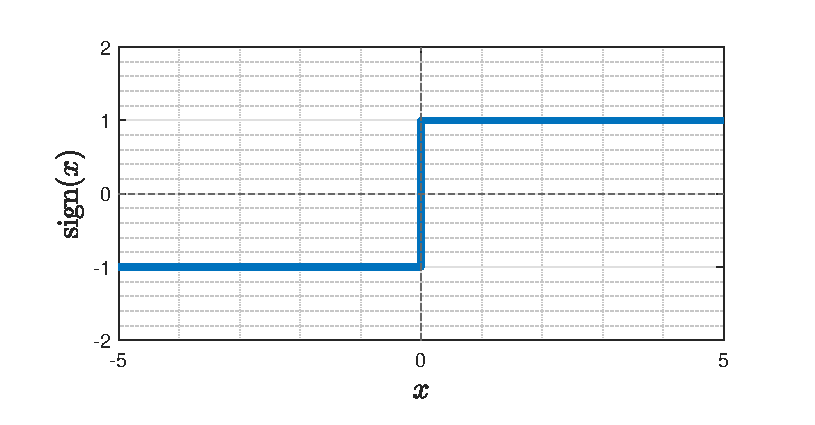
\includegraphics[width=\textwidth]{images/sign.eps}
        \end{figure}
    \end{minipage}
\end{itemize}

\begin{ex}{}
    A ship encounters the superposition of three wave trains, each of which can be modeled as a sinusoidal signal. 
    \[ 
    x(t) = 1+\frac{1}{2}\cos(2\pi t + \phi_{1})+\cos(4\pi t + \phi_{2})+\frac{2}{3}\cos(6\pi t + \phi_{3})
    \]
    With fixed magnitudes for these sinusoids, \textbf{the amplitude of their sum may be quite small or very large, depending on the relative phases.} The implications of phase for the ship, therefore, are quite significant. 
    \begin{figure}[H] 
        \centering
        \includegraphics[width=0.6\textwidth]{images/phase}
    \end{figure}
    (Example adopted from \textbf{Signals and Systems, 2\textsuperscript{nd} Edition}, P424)
\end{ex}

Specifically, for the circuit example above:
\[ 
\lvert H(\omega_{0}) \rvert =  \frac{1}{\sqrt{1+\omega^{2}(RC)^{2} }} = \frac{1}{\sqrt{1+(\frac{\omega}{\omega_{c}})^{2}}} 
\]

\[ 
\angle H(\omega_{0}) = -tan^{-1}(\omega RC) = -tan^{-1}(\frac{\omega}{\omega_{c}})
\]

%==============================================%
\subsection{Fourier Transform of Periodic Signals}
If $x(t)$ is a periodic signal:
\[ 
\mathcal{FT} \{ x(t) \} = 2\pi \sum_{k=-\infty}^{+\infty} c_{k} \delta(\omega - k\omega_{0}) 
\]
where 
\[ 
c_{k}=\frac{1}{T} \int_{-\frac{T}{2}}^{+\frac{T}{2}} x(t) e^{-j\frac{2 \pi k}{T} t} dt 
\]
\begin{dv}{}
    Fourier series of a periodic signal $x(t)$ with period $T$ is:
    \[ 
    x(t) = \sum_{k=-\infty}^{+\infty}c_{k}e^{j \frac{2\pi k}{T}t} \quad \text{with} \quad c_{k} = \frac{1}{T} \int_{-\frac{T}{2}}^{+\frac{T}{2}} x(t)e^{-j \frac{2\pi k}{T}t} dt 
    \]
    By applying linearity property:
    \begin{align*}
    \begin{split}
         X(\omega) 
         &= \mathcal{FT} \bigg\{ \sum_{k=-\infty}^{+\infty}c_{k}e^{j \frac{2\pi k}{T}t} \bigg\} \\
         &=\sum_{k=-\infty}^{+\infty}c_{k} \ \mathcal{FT}\{ e^{jk\omega_{0} t}\}\\
         &= 2\pi \sum_{k=-\infty}^{+\infty} c_{k} \delta(\omega - k\omega_{0}) 
    \end{split}
    \end{align*}
\end{dv}

\subsubsection{Fourier transform of a train of impulses}
\[ 
x(t) = \sum_{n=-\infty}^{+\infty} \delta(t-nT) \ \xrightarrow{\mathcal{FT}}\ X(\omega)=\frac{2\pi}{T}  \ \sum^{+\infty}_{k=-\infty} \delta(\omega-k\omega_{0}) \]
\ where \[ \omega_{0}=\frac{2\pi}{T} 
\]

\begin{dv}{}
    \[ x(t) = \sum_{n=-\infty}^{+\infty} \delta(t-T) \]
    From the definition above, $x(t)$ is periodic with period $T$:
    \[ x(t) = \sum_{k=-\infty}^{+\infty}c_{k}e^{j \frac{2\pi k}{T}t} \quad \text{with} \quad c_{k} = \frac{1}{T} \int_{-\frac{T}{2}}^{+\frac{T}{2}} \delta(t)e^{-j \frac{2\pi k}{T}t} dt = \frac{1}{T} \]
    Thus:
    \[ X(\omega) = \frac{2\pi}{T}\sum_{n=-\infty}^{+\infty}  \delta(\omega-k\omega_{0}) \quad  \text{with}\  \omega_{0}=\frac{2\pi}{T}\]
\end{dv}